% ------------------------------------------------------------------------
%  Cartoon renderings of the two large comparative test molecules, used in
%  Section~\ref{sec:evaluation-results-lin-eq-solver} to argue that geometric
%  complexity -- not atom count -- drives the size of the linear system.
%  Hand-authored; images are RCSB PDB renderings dropped into figures/.
%  1VSZ is shown via its current PDB entry 6CGV, since 1VSZ is obsolete.
%  Include with % ------------------------------------------------------------------------
%  Cartoon renderings of the two large comparative test molecules, used in
%  Section~\ref{sec:evaluation-results-lin-eq-solver} to argue that geometric
%  complexity -- not atom count -- drives the size of the linear system.
%  Hand-authored; images are RCSB PDB renderings dropped into figures/.
%  1VSZ is shown via its current PDB entry 6CGV, since 1VSZ is obsolete.
%  Include with % ------------------------------------------------------------------------
%  Cartoon renderings of the two large comparative test molecules, used in
%  Section~\ref{sec:evaluation-results-lin-eq-solver} to argue that geometric
%  complexity -- not atom count -- drives the size of the linear system.
%  Hand-authored; images are RCSB PDB renderings dropped into figures/.
%  1VSZ is shown via its current PDB entry 6CGV, since 1VSZ is obsolete.
%  Include with % ------------------------------------------------------------------------
%  Cartoon renderings of the two large comparative test molecules, used in
%  Section~\ref{sec:evaluation-results-lin-eq-solver} to argue that geometric
%  complexity -- not atom count -- drives the size of the linear system.
%  Hand-authored; images are RCSB PDB renderings dropped into figures/.
%  1VSZ is shown via its current PDB entry 6CGV, since 1VSZ is obsolete.
%  Include with \input{figures/molecule_shapes}
%  Needs \usepackage{graphicx} and \usepackage{subcaption}.
% ------------------------------------------------------------------------
\begin{figure}[!htb]
\centering
\begin{subfigure}[b]{0.47\textwidth}
    \centering
    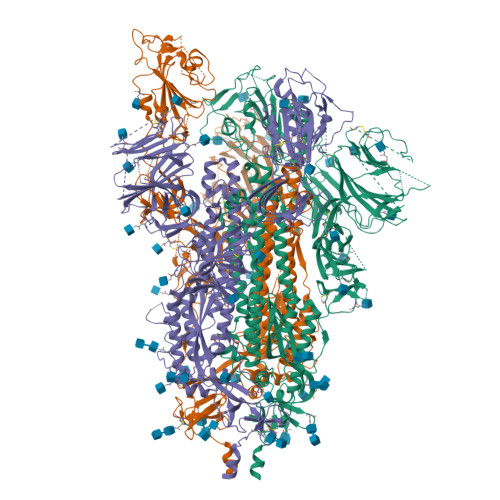
\includegraphics[width=\textwidth]{figures/shape_6vyb.jpeg}
    \caption{6VYB}
    \label{fig:shape-6vyb}
\end{subfigure}
\hfill
\begin{subfigure}[b]{0.47\textwidth}
    \centering
    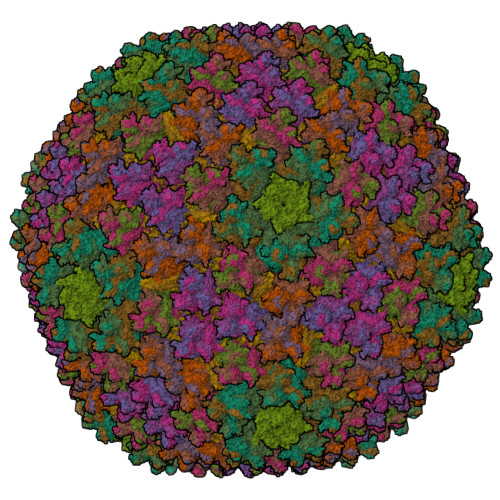
\includegraphics[width=\textwidth]{figures/shape_1vsz.jpeg}
    \caption{6CGV}
    \label{fig:shape-1vsz}
\end{subfigure}
\caption[Molecular shapes of 6VYB and 1VSZ]{Cartoon renderings of the biological assemblies, colored by chain. \textbf{Left:} 6VYB's irregular, elongated spike trimer. \textbf{Right:} the icosahedral capsid of 1VSZ, shown via its current PDB entry 6CGV, since 1VSZ itself is obsolete. Renderings from the RCSB PDB.}
\label{fig:molecule-shapes}
\end{figure}

%  Needs \usepackage{graphicx} and \usepackage{subcaption}.
% ------------------------------------------------------------------------
\begin{figure}[!htb]
\centering
\begin{subfigure}[b]{0.47\textwidth}
    \centering
    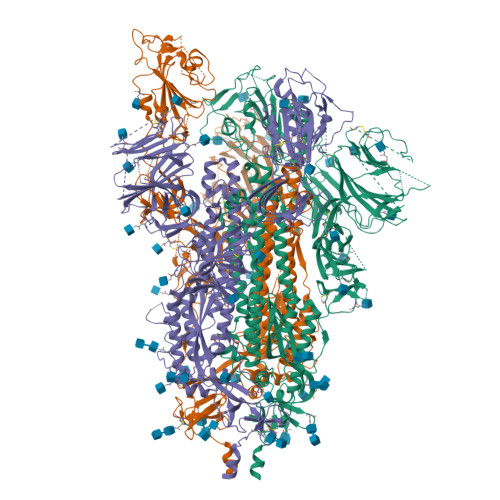
\includegraphics[width=\textwidth]{figures/shape_6vyb.jpeg}
    \caption{6VYB}
    \label{fig:shape-6vyb}
\end{subfigure}
\hfill
\begin{subfigure}[b]{0.47\textwidth}
    \centering
    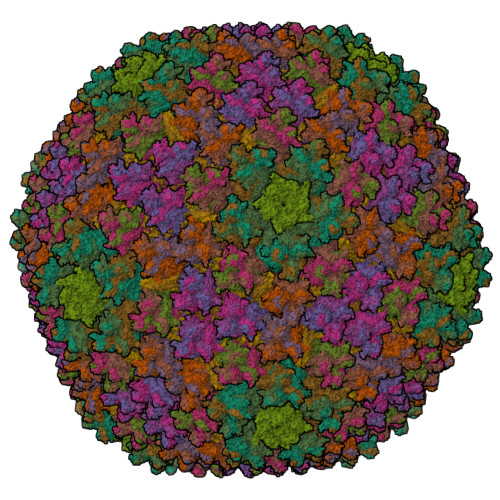
\includegraphics[width=\textwidth]{figures/shape_1vsz.jpeg}
    \caption{6CGV}
    \label{fig:shape-1vsz}
\end{subfigure}
\caption[Molecular shapes of 6VYB and 1VSZ]{Cartoon renderings of the biological assemblies, colored by chain. \textbf{Left:} 6VYB's irregular, elongated spike trimer. \textbf{Right:} the icosahedral capsid of 1VSZ, shown via its current PDB entry 6CGV, since 1VSZ itself is obsolete. Renderings from the RCSB PDB.}
\label{fig:molecule-shapes}
\end{figure}

%  Needs \usepackage{graphicx} and \usepackage{subcaption}.
% ------------------------------------------------------------------------
\begin{figure}[!htb]
\centering
\begin{subfigure}[b]{0.47\textwidth}
    \centering
    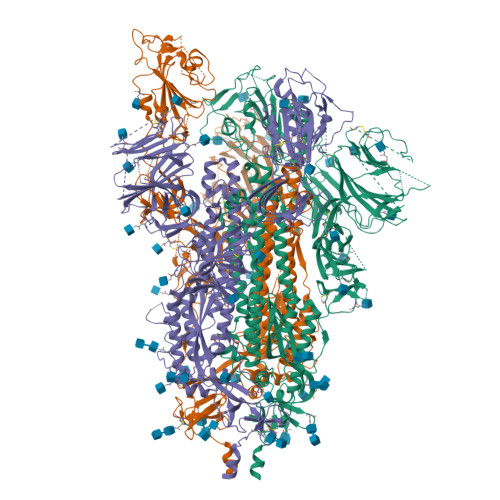
\includegraphics[width=\textwidth]{figures/shape_6vyb.jpeg}
    \caption{6VYB}
    \label{fig:shape-6vyb}
\end{subfigure}
\hfill
\begin{subfigure}[b]{0.47\textwidth}
    \centering
    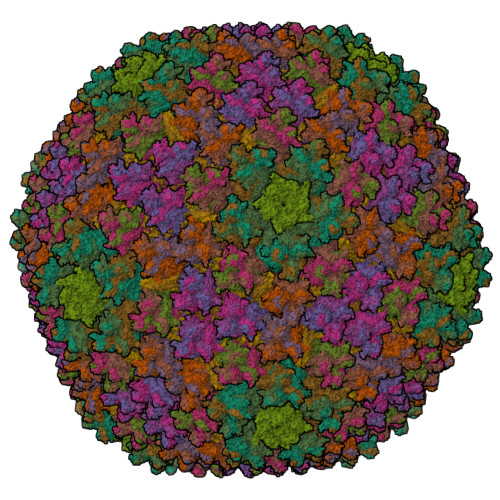
\includegraphics[width=\textwidth]{figures/shape_1vsz.jpeg}
    \caption{6CGV}
    \label{fig:shape-1vsz}
\end{subfigure}
\caption[Molecular shapes of 6VYB and 1VSZ]{Cartoon renderings of the biological assemblies, colored by chain. \textbf{Left:} 6VYB's irregular, elongated spike trimer. \textbf{Right:} the icosahedral capsid of 1VSZ, shown via its current PDB entry 6CGV, since 1VSZ itself is obsolete. Renderings from the RCSB PDB.}
\label{fig:molecule-shapes}
\end{figure}

%  Needs \usepackage{graphicx} and \usepackage{subcaption}.
% ------------------------------------------------------------------------
\begin{figure}[!htb]
\centering
\begin{subfigure}[b]{0.47\textwidth}
    \centering
    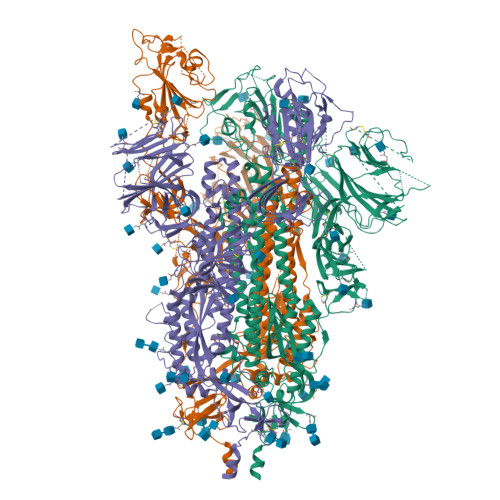
\includegraphics[width=\textwidth]{figures/shape_6vyb.jpeg}
    \caption{6VYB}
    \label{fig:shape-6vyb}
\end{subfigure}
\hfill
\begin{subfigure}[b]{0.47\textwidth}
    \centering
    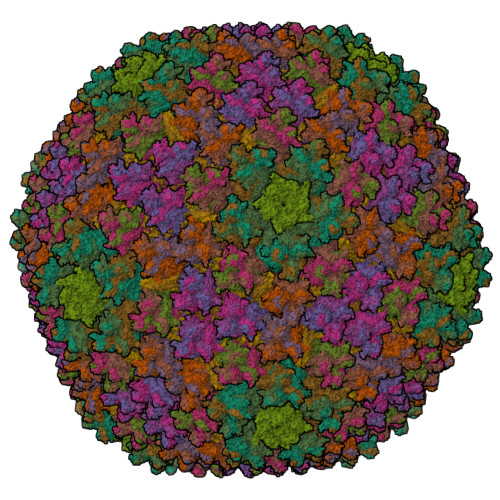
\includegraphics[width=\textwidth]{figures/shape_1vsz.jpeg}
    \caption{6CGV}
    \label{fig:shape-1vsz}
\end{subfigure}
\caption[Molecular shapes of 6VYB and 1VSZ]{Cartoon renderings of the biological assemblies, colored by chain. \textbf{Left:} 6VYB's irregular, elongated spike trimer. \textbf{Right:} the icosahedral capsid of 1VSZ, shown via its current PDB entry 6CGV, since 1VSZ itself is obsolete. Renderings from the RCSB PDB.}
\label{fig:molecule-shapes}
\end{figure}
